\documentclass{article}

\usepackage{fancyhdr} % Required for custom headers
\usepackage{lastpage} % Required to determine the last page for the footer
\usepackage{extramarks} % Required for headers and footers
\usepackage[usenames,dvipsnames]{color} % Required for custom colors
\usepackage{graphicx} % Required to insert images
\usepackage{listings} % Required for insertion of code
\usepackage{courier} % Required for the courier font
\usepackage{multirow}
\usepackage{hyperref}
\usepackage{graphicx} 
\usepackage[utf8]{inputenc}

% Margins
\topmargin=-0.45in
\evensidemargin=0in
\oddsidemargin=0in
\textwidth=6.5in
\textheight=9.0in
\headsep=0.25in

\linespread{1.1} % Line spacing

%----------------------------------------------------------------------------------------
%	CODE INCLUSION CONFIGURATION
%----------------------------------------------------------------------------------------

\definecolor{MyDarkGreen}{rgb}{0.0,0.4,0.0} % This is the color used for comments
\lstloadlanguages{c} % Load Perl syntax for listings, for a list of other languages supported see: ftp://ftp.tex.ac.uk/tex-archive/macros/latex/contrib/listings/listings.pdf
\lstset{language=[sharp]c, % Use Perl in this example
        frame=single, % Single frame around code
        basicstyle=\small\ttfamily, % Use small true type font
        keywordstyle=[1]\color{Blue}\bf, % Perl functions bold and blue
        keywordstyle=[2]\color{Purple}, % Perl function arguments purple
        keywordstyle=[3]\color{Blue}\underbar, % Custom functions underlined and blue
        identifierstyle=, % Nothing special about identifiers                                         
        commentstyle=\usefont{T1}{pcr}{m}{sl}\color{MyDarkGreen}\small, % Comments small dark green courier font
        stringstyle=\color{Purple}, % Strings are purple
        showstringspaces=false, % Don't put marks in string spaces
        tabsize=5, % 5 spaces per tab
        %
        % Put standard Perl functions not included in the default language here
        morekeywords={rand},
        %
        % Put Perl function parameters here
        morekeywords=[2]{on, off, interp},
        %
        % Put user defined functions here
        morekeywords=[3]{test},
       	%
        morecomment=[l][\color{Blue}]{...}, % Line continuation (...) like blue comment
        numbers=left, % Line numbers on left
        firstnumber=1, % Line numbers start with line 1
        numberstyle=\tiny\color{Blue}, % Line numbers are blue and small
        stepnumber=5 % Line numbers go in steps of 5
}

\newcommand{\horrule}[1]{\rule{\linewidth}{#1}}

% Creates a new command to include a perl script, the first parameter is the filename of the script (without .pl), the second parameter is the caption
\newcommand{\perlscript}[2]{
\begin{itemize}
\item[]\lstinputlisting[caption=#2,label=#1]{#1.cs}
\end{itemize}
}

\begin{document}

\begin{tabular}{l l}
 & Facultad de Ingenieria \\
 & Ing. en Sistemas \\
 & Informatica 1 \\
 & Prof. Ernesto Rodriguez - \href{mailto:erodriguez@unis.edu.gt}{erodriguez@unis.edu.gt} \\
\end{tabular}
\\\\\\

\begin{center}
        \horrule{0.5pt}
        \huge{Examen Parcial \#1} \\
        \large{Tiempo de resoluci\'on: 90 minutos} \\
        \horrule{1pt}
\end{center}

\emph{Instrucciones: Responder las preguntas que se presentan a continuaci\'on y hacer los ejercicios que se presenten
        a continuaci\'on.}


\section{Pregunta \#1 (20\%)}
El famoso matematico Euler hizo la siguiente pregunta: ¿Es possible curzar todos los puentes
de K\"onigsberg sin pasar dos veces por el mismo puente? A continuaci\'on se muestra un
mapa de los puentes de K\"onigsberg:

Su tarea es crear un grafo a partir de estos puentes. Para ello debe:
\begin{itemize}
        \item{Definir el conjunto de nodos}
        \paragraph{Resoluc\'on}
       \ \\ \ siendo $\rightarrow$ $1 = isla 1, 2 = isla 2, 3 = isla 3, 4 = isla 4$
        \ \\ \ $[(1) (2) (3) (4)]$
        \item{Definir el conjunto de vertices}
        \[
           \left\{
        \begin{array}{l l}
          \ \\ \ $(1,2) (1,3) (1,4)$
       \ \\ \  $(2,1) (2,3)$
       \ \\ \ $(3,1) (3,2) (3,4)$
       \ \\ \ $(4,1) (4,3)$\\
        \end{array}
        \right.
        \]
\paragraph{Grafo}
\ \\ \
  \begin{figure}
	\begin{center}
		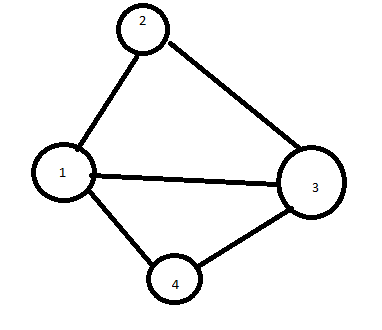
\includegraphics[width=0.5\textwidth]{gr.png}
		\caption{Grafo}
	\end{center}
\end{figure}
\ \\ \
\ \\ \
\ \\ \
\ \\ \
\ \\ \
\ \\ \
\ \\ \
\ \\ \

\section*{Pregunta \#2 (20\%)}
Demostrar utilizando inducci\'on que la formula de Gauss para sumatorias es correcta:
\[
        \sum_{i=1}^{n}{i}=\frac{n(n+1)}{2}
\]
donde $\sum_{i=1}^{n}i=1+2+3+4+\ \ldots\ +n$.
\\\\
Para esta demostraci\'on, su caso base debe ser
$n=1$ en vez de $n=0$. Sin embargo, la demostraci\'on
del caso inductivo procede de la misma forma que
se ha estudiado en clase.
\ \\ \ \paragraph{Resoluc\'on}
\ \\ \ $ s = 1+2+3.... + (n-1) +n $
\ \\ \ $s= n+(n-1)+(n-2)+...+2+1$
\ \\ $\oplus$\rule[0mm]{40mm}{0.1mm}
\ \\ \ $2s=(n+1)+(n+1)+(n+1)..$
\ \\ \ $2s=n(n+1)$
\ \\ \ $s=\frac{n(n+1)}{2}$

\section*{Pregunta \#3 (20\%)}
Definir inductivamente la funcion $\sum(n)$ para numeros naturales unarios la cual tiene
el efecto de calcular la suma de $1$ hasta $n$. En otras palabras:
\[
        \sum(n)=1+2+3+4+\ \ldots\ +n
\]
Puede apoyarse de la suma $\oplus$ de numeros naturales unarios para su definici\'on:
\[
        a\oplus b =
                \left\{
                        \begin{array}{ll}
                                b  & \mbox{si } a = 0 \\
                                s(i\oplus b) & \mbox{si } a = s(i)
                        \end{array}
                \right.
\]
\paragraph{Resoluci\'on}
\ \\ \ Aplicando la formula de Gauss
\ \\ \ $\sum s(0)= \frac{(s(0))(s(0)\oplus s(0))}{s(s(0))}$
\ \\ \ $\sum s(0)= \frac{s(0)(s(s(0)))}{s(s(0))}$
\ \\ \ $\sum s(0)= \frac{s(s(0))}{s(s(0))}$
\ \\ \ $\sum s(0)= s(0)$
\section*{Pregutna \# 4 (20\%)}
Demostrar por medio de inducci\'on la comutatividad de la suma de
numeros naturales unarios: $a\oplus b = b\oplus a$
\paragraph{Resoluci\'on}
\ \\ \ $\rightarrow$ $a=s(0)
\ \\ \ $$\rightarrow$ $ b=s(s(0)$
\ \\ \ $a\oplus b = b\oplus a$
\ \\ \ $s(0)\oplus s(s(0) = s(s(0)  \oplus s(0)$
\ \\ \ $s(s(0) \oplus s(0) = s(ss(0) \oplus 0$
\ \\ \ $s(ss(0) \oplus 0 = s(ss(0)$
\ \\ \ $s(ss(0) = s(ss(0)$
\ \\ \ $\rightarrow$ Si son iguales
\section*{Pregunta \#5 (20\%)}
Dada la funci\'on $a\geq b$ para numeros naturales unarios:
\[
        a\geq b =
                \left\{
                        \begin{array}{ll}
                                s(o)  & \mbox{si } b = o \\
                                o & \mbox{si } a = o \\
                                i\geq j & \mbox{si } a = s(i)\ \&\ b = s(j)
                        \end{array}
                \right.
\]
Demostrar utilizando inducci\'on que $((n\oplus n)\geq n) = s(o)$. Puede
hacer uso de la asociatividad y comutabilidad de la suma de numeros
unarios para su demostraci\'on.
\paragraph{Resoluci\'on}
\ \\ \ $\rightarrow$ $n=s(0)$
\ \\ \ $((s(0)$ $\oplus$ $ s(0)$ $\geq$ $ s(0)) = s(0)$
\ \\ \ $s(s(0)) \geq s(0) = s(0)$
\ \\ \ $s(s(0))-s(0) \geq 0 = s(0)$
\ \\ \ $s(0) \geq 0 = s(0)$
\ \\ \ $0 \leq s(0) = s(0)$
\end{itemize}
\end{document}